\IfFileExists{ci.tex}{
    \input{ci.tex}
}{}
\documentclass[
    ngerman,
    color=3b,
    % dark_mode, % uncomment for dark mode
    % load_common, % läd oft benutzte Pakete, erhöht aber die Compile-Time drastisch
    summary,
    %twosided,
    boxarc,
    main,
    fleqn,
    leqno,
]{rubos-tuda-template}

\usepackage{datetime}

%% Summary settings--%%
\title[AuPL]{Aussagen und Prädikatenlogik}
\subtitle{Aufgabenguide}
\semester{SoSe 2022}
\fachbereich{Informatik}
\author{Ruben Deisenroth}
\date{\today,~\currenttime~Uhr}
% \version{1.0-Snapshot}
\termOrder{printAuthor,printSemester,,%
    ,printFachbereich,printDate}

\newcommand*\cleartoleftpage{%
    \clearpage
    \ifodd\value{page}\hbox{}\newpage\fi
}

%% Style stuff--%%
\ExplSyntaxOn

\ConfigureHeadline{
    headline={\centering
        \textbf{\sffamily\g_ptxcd_shorttitle_tl\space{}Aufgabenguide}
        \space{}von\space{}
        \seq_use:Nnnn \g_ptxcd_author_seq {~\authorandname{}~} {,~} {~\authorandname{}~}}
}
\ExplSyntaxOff

\usepackage{forest}
\usepackage[fleqn]{nccmath}
\usepackage{placeins}
\usepackage{ebproof}
\usepackage{prftree}
\newcommand{\infer}[2]{\prftree{#2}{#1}}
\usepackage[
    color=accentcolor,
    textcolor=white,
    textwidth=.8cm,
    textsize=small,
    loadshadowlibrary,
]{todonotes}

% \usepackage{icomma}
\usepackage{tikz}
\usetikzlibrary{shapes.geometric,calc,arrows.meta}
\usetikzlibrary{tikzmark}
\ExplSyntaxOn
\def\maxstars{5}
% #1: Amount of stars to be filled
\tikzset{
    scorestar/.style={
        draw,
        star,
        star~points=5,
        star~point~ratio=2.25,
        inner~sep=1.3pt,
        anchor=outer~point~3,
    },
    scorestarempty/.style={
        scorestar,
        fill=none,
    },
    scorestarfill/.style={
        scorestar,
        fill=accentcolor,
    },
}
\DeclareDocumentCommand{\stars}{m}
{
    \begin{tikzpicture}[baseline]
        \fp_step_inline:nnnn {1} {1} {\maxstars}{
            % first, draw the empty stars as a background to potentially be filled
            \node[scorestarempty] (star##1) at (##1*1.75ex, 0) {};
            % Check if the current step is smaller than the amount of stars to be filled. To account for partially filled stars, we check instead if the current step is smaler than the amount of stars to be filled plus 1, so partially filled stars are also counted.
            \fp_compare:nT {##1<(#1+1)} {
                % Check if The remainder of stars to be filled is smaller than 0. If So, ##1 will be greater than #1 since we "overshoot".
                \fp_compare:nTF {##1 > #1} {
                    %
                    \begin{scope}
                        \clip
                        ($(star##1.outer~point~3)!(star##1.outer~point~2)!(star##1.outer~point~4)$)
                        rectangle
                        ($(star##1.outer~point~2 |- star##1.outer~point~1)!\fp_eval:n {#1 - (##1-1)}!(star##1.outer~point~1 -| star##1.outer~point~5)$);
                        \node[scorestarfill] (starcol##1) at (##1*1.75ex, 0) {};
                    \end{scope}
                } {
                    \node[scorestarfill] (starcol##1) at (##1*1.75ex, 0) {};
                }
            }
        }
    \end{tikzpicture}%
}
\ExplSyntaxOff
\DeclareDocumentCommand{\exstats}{mm}{
    \par\noindent\hfill\fatsf{Schwierigkeit:\stars{#1}}, \fatsf{Benötigte Zeit}: #2\hfill\mbox{}\par\noindent
}

%% Begin of document--%%
\begin{document}

    %--Titelseite--
    \label{toc}\maketitle{}
    \section{Vorwort}
    Du befindest dich gerade mitten in der AuPL Prüfung, hast keinen Plan von den Aufgaben und blätterst verzweifelt durch dein ganzes Ausgedrucktes Zeug, und eventuell bist du bei diesem Zettel gelandet, den irgend so ein rando auf dem Geekhub hochgeladen hat? Dann musst du jetzt nicht mehr weitersuchen, denn dieses Aufgabenguide ist genau das, was du brauchst. Hier findest du zu jedem Aufgabentyp die notwendigen Definitionen, ein idiotensicheres -- auf Zeit optimiertes -- Lösungsguide mit Beispielen, und eine Einschätzung für Schwierigkeitsgrad und Zeitbedarf. Aber was tust du denn da bitte?! Du hast doch gar keine Zeit mehr, also fang endlich an zu Blättern, und schau am Besten im \hyperref[toc]{Inhaltsverzeichnis} auf Seite \pageref{toc} vorbei.

    Du bist ja immernoch hier? Nagut, dann wünsche ich dir viel Erfolg bei der Prüfung, und hoffe, dass du mit diesem Aufgabenguide deine Prüfung bestehst!
    \tableofcontents %Inhaltsverzeichnis

    %---Beginn Der Zusammenfassung---%


    \vspace{\fill}
    %medal
    \begin{tikzpicture}[ultra thick,black!\IfDarkModeTF{8}{6}0!orange!\IfDarkModeTF{5}{4}0!yellow, overlay]
        \coordinate (c) at ([xshift=6cm,yshift=-8.5cm]current page.north west);
        \draw[teal,line width=.8cm,-{Triangle Cap[reversed]}] (c) -- ($(c)+(250:3cm)$);
        \draw[teal,line width=.8cm,-{Triangle Cap[reversed]}] (c) -- ($(c)+(290:3cm)$);
        \filldraw[draw=\thepagecolor] (c) circle (1.5cm);
        \node[white,align=center, text width=2.1cm,draw=\thepagecolor,circle,font=\footnotesize\sffamily\bfseries, inner sep=0pt] at (c) {Unvollständigkeitsgarantie};
    \end{tikzpicture}
    \mbox{}
    \cleartoleftpage{}
    \section{Aussagenlogik}
    \subsection{KNF und DNF}
    \exstats{.5}{2min}
    \begin{definition}[DNF]\label{dnf} (Diskunktive Normalenform)
        Veroderung von Verundungen: $\{\{x\land y\land\dots\}\lor\{a\land b\land\dots\}\lor\dots\}$
    \end{definition}
    \begin{definition}[KNF]\label{knf} (Konjunktive Normalenform)
        Verundung von Veroderungen: $\{\{x\lor y\lor\dots\}\land\{a\lor b\lor\dots\}\land\dots\}$
    \end{definition}
    \begin{tipp}
        Nach De-Morgan: Strich über die Einzelnen Buhstaben, $\land$ und $\lor$ vertauschen is äquivalent zum Ursprung:\\ $a\land b = \overline{a}\lor \overline{b}$
    \end{tipp}
    \subsubsection{aus Wahrheitstabelle}
    \paragraph{Vorgehen} Zuerst musst du die Klausel+Spalte erstellen.
    Dazu einfach bei wahren Zeilen die Variablen verunden, und bei falschen Zeilen den Wahrheitswert der Variablen \fatsf{negieren} und dann die Variablen verodern. Für DNF dann einfach die Terme der Wahren Spalten verodern, für KNF die Terme der Falschen Spalten verunden.

    \begin{table}[ht!]
        \rowcolors{2}{\thepagecolor}{fgcolor!10!\thepagecolor}
        \centering
        \begin{tabular}{c|c|c|c|l}
            p & q & r & $(q\lor r)\rightarrow(p\land\lnot (p\land r))$ & Klausel                                                                                      \\
            \hline
            0 & 0 & 0 & \cellcolor{green!20!\thepagecolor} 1           & \cellcolor{green!20!\thepagecolor}$\lnot p\land \lnot q\land \lnot r$ \tikzmark{truethtabk1} \\
            0 & 0 & 1 & \cellcolor{red!20!\thepagecolor} 0             & \cellcolor{red!20!\thepagecolor}$p\lor q\lor\lnot r$                  \tikzmark{truethtabk2} \\
            0 & 1 & 0 & \cellcolor{red!20!\thepagecolor} 0             & \cellcolor{red!20!\thepagecolor}$p\lor \lnot q\lor r$                 \tikzmark{truethtabk3} \\
            0 & 1 & 1 & \cellcolor{red!20!\thepagecolor} 0             & \cellcolor{red!20!\thepagecolor}$p\lor \lnot q\lor \lnot r$         \tikzmark{truethtabk4}   \\
            1 & 0 & 0 & \cellcolor{green!20!\thepagecolor} 1           & \cellcolor{green!20!\thepagecolor}$p\land \lnot q\land \lnot r$     \tikzmark{truethtabk5}   \\
            1 & 0 & 1 & \cellcolor{red!20!\thepagecolor} 0             & \cellcolor{red!20!\thepagecolor}$\lnot p\lor q\lor \lnot r$       \tikzmark{truethtabk6}     \\
            1 & 1 & 0 & \cellcolor{green!20!\thepagecolor} 1           & \cellcolor{green!20!\thepagecolor}$p\land \lnot q\land r$         \tikzmark{truethtabk7}     \\
            1 & 1 & 1 & \cellcolor{red!20!\thepagecolor} 0             & \cellcolor{red!20!\thepagecolor}$\lnot p\lor \lnot q\lor \lnot r$     \tikzmark{truethtabk8}
        \end{tabular}
        \caption{Wahrheitstabelle für $\varphi=(q\lor r)\rightarrow(p\land\lnot (p\land r))$}
        \label{tab:truethtab}
    \end{table}

    \textcolor{green!80!black}{\textbf{DNF:}} $(\lnot p\land \lnot q\land \lnot r)\lor(p\land \lnot q\land \lnot r)\lor(p\land \lnot q\land r)$\tikzmark{dnf}\\
    \textcolor{red}{\textbf{KNF:}} $(p\lor q\lor\lnot r)\land(p\lor \lnot q\lor r)\land(p\lor \lnot q\lor \lnot r)\land(\lnot p\lor q\lor \lnot r)\land(\lnot p\lor \lnot q\lor \lnot r)$\tikzmark{knf}
    \begin{tikzpicture}[remember picture, overlay, thick,-Latex]
        \begin{scope}[green!80!black]
            \node[circle,draw] (dnfcenter) at ($(pic cs:truethtabk1)+(2cm,-.5cm)$) {$\lor$};
            \foreach \i in {1,5, 7}{
                \draw (pic cs:truethtabk\i) -- (dnfcenter);
            }
            \draw (dnfcenter) |- ([yshift=.5ex]pic cs:dnf);
        \end{scope}
        \begin{scope}[red]
            \node[circle,draw] (knfcenter) at ($(pic cs:truethtabk4)+(3cm,0cm)$) {$\land$};
            \foreach \i in {2,3,4,6,8}{
                \draw (pic cs:truethtabk\i) -- (knfcenter);
            }
            \draw (knfcenter) |- ([yshift=.5ex]pic cs:knf);
        \end{scope}
    \end{tikzpicture}
    \begin{anmerkung}
        Die DNF ist \textbf{nicht} immer kürzer oder angenehmer, sondern nur in diesem Beispiel.
    \end{anmerkung}
    \clearpage
    \subsection{Resolutionsverfahren}
    \exstats{1.5}{3min}
    \begin{definition}[Literal]
        Buchstabe mit oder ohne Negation, z.B.: $a$ oder $\lnot a$ (aber nicht sowas: $a\rightarrow{}b$)
    \end{definition}
    \begin{definition}[Klausel]
        Menge mit einzelnen Literalen, KNF Glied -- Komma = $\lor$ z.B.: $\{\lnot a, b,\lnot c, d\}$  (aber nicht $\{a\rightarrow{}b,\lnot d\}$)
    \end{definition}
    \begin{definition}[Klauselmenge]
        Menge von Klauseln, in KNF -- aber innerhalb der Glieder wird $\lor$ durch ein Komma und außerhalb der Glieder wird $\land$ ebenfalls durch ein Komma ersetzt.
    \end{definition}
    \paragraph{Vorgehen}
    \begin{steps}
        \item Unerfüllbarkeitsaussage (falls noch nicht getan): wenn da steht du sollst die Allgemeingültigkeit der Formel zeigen, musst du diese zunächst durch negieren (\enquote{in eine Unerfüllbarkeitsaussagen umwandeln}).
        \item Formel in \hyperref[knf]{KNF} umwandeln, falls noch nicht in KNF. (Definition KNF auf \pagename~\pageref{knf})
        \item Klauselmenge aufschreiben: einfach KNF so wie in der Definition auf \pageref{knf}, nur ersetzen wir die \enquote{$\lor$} und \enquote{$\land$} durch Kommas \enquote{$,$}.
        \item Wir spielen Minecraft, und craften jetzt die einzelnen Klauseln so zusammen, dass wir die leere Klausel erhalten. Was sich logisch widerspricht, löst sich auf. Dabei fängst du am Besten mit der größten Klausel an, und schaust, dass du eine findest, die möglichst viele Teile davon auflösen kann, bis du irgendwann die leere Menge hat, die man mit $\Box$ beschreibt.
        \item Falls die Leere Menge nicht herleitbar ist, ist die Klauselmenge erfüllbar.
    \end{steps}
    \paragraph{Beispiel}
    Beweisen von Folgerungsbeziehung $\left\{p,p\rightarrow q, \left(p\rightarrow q\right)\rightarrow\left(q \rightarrow r\right)\right\}\models r$, also zeigen der Unerfüllbarkeit von $\lnot(\left\{p,p\rightarrow q, \left(p\rightarrow q\right)\rightarrow\left(q \rightarrow r\right)\right\}\models r)$.
    Die Klauselmenge liest man dann leicht ab: $\{\{p\},\{\lnot p, q\},\{p,\lnot q,r\},\{\lnot q, r\},\{\lnot r\}\}$
    \begin{center}
        \begin{forest}
            for tree={
            grow'=north,
            calign=first,
            content format={\ensuremath{\left\{\forestoption{content}\right\}}},
            edge={thick,Latex-},
            }
            [\Box, content format={\ensuremath{\forestoption{content}}}[r[q[p][{\lnot p, q}]][{\lnot q, r}]][{\lnot r}]]
        \end{forest}
    \end{center}
    \subsubsection{Einheitsresulotion}
    Selbes Wie normale Resolution, aber mit Hornklauseln, und man darf nur mit einelementigen Klauseln ableiten.
    \clearpage
    \subsection{Hornklausel-Erfüllbarkeitstest/Minimale erfüllende Interpretation}
    \exstats{2}{3min}
    \begin{definition}[Literal]
        Buchstabe mit oder ohne Negation, z.B.: $a$ oder $\lnot a$ (aber nicht sowas: $a\rightarrow{}b$)
    \end{definition}
    \begin{definition}[Klausel]
        Menge mit einzelnen Literalen, KNF Glied -- Komma = $\lor$ z.B.: $\{\lnot a, b,\lnot c, d\}$  (aber nicht $\{a\rightarrow{}b,\lnot d\}$)
    \end{definition}
    \begin{definition}[Hornklausel]
        Eine Klausel $\mathcal{C}$ mit \textbf{höchstens} einem positiven Literal.
        \begin{itemize}
            \item Positive Hornklausel: $\mathcal{C}$ besteht nur aus einem positiven Literal
            \item negative Hornklausel: $\mathcal{C}$ enthält kein positives Literal
        \end{itemize}
    \end{definition}
    \begin{definition}[Klauselmenge]
        Menge von Klauseln, in KNF -- aber innerhalb der Glieder wird $\lor$ durch ein Komma und außerhalb der Glieder wird $\land$ ebenfalls durch ein Komma ersetzt.
        \begin{itemize}
            \item Hornklauselmenge: Klauselmenge wo alle Klauseln Hornklauseln sind
        \end{itemize}
    \end{definition}
    \paragraph{Vorgehen}
    \begin{steps}
        \item Wir fangen erst mal mit der Leeren Menge an: $\mathcal{X}_0=\emptyset$
        \item Jetzt suchen wir alle Positiven Hornklauseln und fügen sie zu unserer Menge X hinzu: $\mathcal{X}{n+1}=\{\dots\}$
        \item Falls keine Positiven Hornklauseln mehr existieren, springe zu Schritt 5
        \item Falls doch \enquote{Streichen} wir aus allen anderen Klauseln die negation der zu $\mathcal{X}$ neu hinzugekommenen Variablen einfach raus, falls diese vorkommen und Springen zu Schritt 2 mit der neuen Klauselmenge
        \item Jetzt haben wir $\mathcal{X}_\infty$ berechnet, das ist die minimale Belegung. Wenn wir jetzt jede Klausel (unveränderten) Klauselmenge durchgehen, und schauen ob diese erfüllt ist, wenn wir alle Literale von $x$ auf 1 und alle anderen auf $0$ setzen. Falls ja ist die Formel erfüllbar, falls nein ist sie unerfüllbar.
    \end{steps}
    \paragraph{Beispiel}\mbox{}

    $H = \{\{\lnot p, \lnot t, s\}, \{p\}, \{\lnot p, \lnot q, r\}, \{t\}, \{\lnot p, \lnot s, q\}, \{\lnot s, \lnot r, t\}, \{\lnot p, \lnot u, r\}, \{\lnot u\}, \{\lnot q\}\}$
    \begin{ceqn}
        \begin{align*}
            \mathcal{X}_0             & = \emptyset                                                      \\
            \mathcal{X}_1             & = \{p, t\}                                                       \\
            \mathcal{X}_2             & = \{p, t, s\}                                                    \\
            \mathcal{X}_3             & = \{p, t, s, q\}                                                 \\
            \mathcal{X}_4             & = \{p, t, s, q, r\}                                              \\
            \mathcal{X}_5             & = \{p, t, s, q, r\}                                              \\
            \mathrm{Da}~\mathcal{X}_5 & = \mathcal{X}_4 ~\mathrm{ist}~\mathcal{X}_4 = \mathcal{X}_\infty
        \end{align*}
    \end{ceqn}

    Die negative Klausel $\{\lnot q\}$ ist unter der minimalen Interpretation falsch und somit ist $H$ unerfüllbar.
    \clearpage
    \subsection{Modell aufstellen}
    \exstats{2.5}{3min}
    Ein Modell für eine Signatur $\sigma$ braucht eine Trägermenge, und alle Relationen, Funktionen und Konstanten aus $\sigma$. z.B. für $\sigma = \{+,\cdot,0,1\}$ wäre ein Mögliches Modell: $\mathcal{N}:=(\mathbb{N},+^{\mathbb{N}},\cdot^{\mathbb{N}},0,1)$

    Meistens musst du allerdings die Relationen oder Funktionen noch so definieren, dass gewisse Eigenschaften erfüllt sind. Honestly: hier am Besten zu Übungslösungen blättern für Inspiration.

    \subsection{AL-Formeln aufstellen}
    \exstats{1}{2min}
    \begin{definition}[Aussagenlogik]\mbox{}
        \begin{itemize}
            \item Variablen (z.B. $v_0, v_1, x, y,\dots $)
            \item Logische Operatoren \enquote{$\lnot$} (nicht), \enquote{$\land$} (und), \enquote{$\lor$} (oder),
                \enquote{$\rightarrow{}$} (impliziert), und \enquote{$\leftrightarrow$} (genau dann wenn)
        \end{itemize}
    \end{definition}

    \subsection{semantisch Gültigkeit einer Regel beweisen}
    \exstats{3}{4min}
    \begin{definition}[Prämisse]
        Das was über dem Strich steht, oft gibt es mehr als eine Prämisse, manchmal gar keine.
    \end{definition}
    \begin{definition}[Konklusion]
        Das was unter dem Strich steht.
    \end{definition}
    \begin{definition}[$\vdash$]
        Lies es so: alles was links von $\vdash$ steht wird verundet, und alles was rechts von $\vdash$ steht wird verodert. Stell dir $\vdash$ wie eine Implikation vor, das heißt entweder die linke Seite ist falsch, oder die rechte Seite ist wahr.
    \end{definition}
    \paragraph{Vorgehen}
    \begin{steps}
        \item Schreib den Satz: \enquote{Angenommen die Prämissen sind Gültig, wir müssen zeigen, dass dann die Konklusion auch allgemeingültig ist.} ab.
        \item Jetzt schau dir die linke Seite der Konklusion an (alles vor $\vdash$). Am Besten erst mal den Fall betrachten, bei dem das falsch ist, in dem Fall \enquote{sind wir fertig.}
        \item Danach alle weiteren Fälle durchgehen, und immer im Kopf behalten, dass die Prämissen allgemeingültig sind.
    \end{steps}
    \paragraph{Wichtige Schreibweisen} \begin{itemize}
        \item $\mathfrak{I}\models\varphi$ bedeutet: $\mathfrak{I}$ ist ein Modell von $\varphi$. (also $\mathfrak{I}$ ist eine erfüllende Belegung von $\varphi$)
        \item Sowas wie: Da $\Gamma\vdash \varphi\rightarrow\psi ,\delta$ allgemeingültig ist, gibt es eine Formel $\delta\in\Delta\cup\{\varphi\rightarrow\psi\}$
            mit $\mathfrak{I}\in\delta$.
        \item $(\lnot \rho)^{\mathfrak{I}}=0$.
        \item Am Ende nach dem letzten Punkt einen $\Box$ zeichnen, um zu zeigen, dass wir sogar dafür genügend Zeit hatten. (alternativ qed. schreiben, um schlau zu wirken oder so)
    \end{itemize}
    \clearpage
    \subsection{Regel im AL-Sequenzenkalkül ableiten}
    \exstats{2.5}{3-6 min, je nach Länge der Regel}
    \begin{definition}[Prämisse]
        Das was über dem Strich steht, oft gibt es mehr als eine Prämisse, manchmal gar keine.
    \end{definition}
    \begin{definition}[Konklusion]
        Das was unter dem Strich steht.
    \end{definition}
    \begin{definition}[$\vdash$]
        Lies es so: alles was links von $\vdash$ steht wird verundet, und alles was rechts von $\vdash$ steht wird verodert. Stell dir $\vdash$ wie eine Implikation vor, das heißt entweder die linke Seite ist falsch, oder die rechte Seite ist wahr.
    \end{definition}
    \begin{definition}[Regel (Ax)]
        Die Eierlegende Wollmilchsau, die uns quasi alle Regeln erstellen lässt, solange auf der rechten Seite irgendwann mal das Gleiche vorkommt, wie auf der Linken Seite.
    \end{definition}
    \begin{figure}[ht!]
        \centering%
        \begin{subfigure}[c]{.55\textwidth}
            \centering
            \begin{tabular}{| l l l l |}
                \hline
                (Ax)          & \infer{\Gamma, \varphi \vdash \Delta, \varphi}{\phantom{I}}                                                     &               &                                                                                                                  \\
                (0-Ax)        & \infer{\Gamma, 0 \vdash \Delta}{}                                                                               & (1-Ax)        & \infer{\Gamma \vdash \Delta, 1}{\phantom{I}}                                                                     \\
                $ (\lnot L) $ & \infer{\Gamma, \lnot \vdash \Delta}{\Gamma \vdash \Delta, \varphi}                                              & $ (\lnot R $) & \infer{\Gamma \vdash \Delta, \lnot \varphi}{\Gamma, \varphi \vdash \Delta}                                       \\
                $ (\lor L) $  & \infer{\Gamma, \varphi \lor \psi \vdash \Delta}{\Gamma, \varphi \vdash \Delta \quad \Gamma, \psi \vdash \Delta} & $ (\lor R) $  & \infer{\Gamma \vdash \Delta, \varphi \lor \psi}{\Gamma \vdash \Delta, \varphi, \psi}                             \\
                $ (\land L) $ & \infer{\Gamma, \varphi \land \psi \vdash \Delta}{\Gamma, \varphi, \psi \vdash \Delta}                           & $ (\land R) $ & \infer{\Gamma \vdash \Delta, \varphi \land \psi}{\Gamma \vdash \Delta, \varphi \quad \Gamma \vdash \Delta, \psi} \\
                \hline
            \end{tabular}
            \caption{Schlussregeln in $ \mathcal{SK} $}
            \label{fig:al:skregeln}
        \end{subfigure}%
        \begin{subfigure}[c]{.45\textwidth}
            \centering
            \begin{tabular}{| l l |}
                \hline
                (modus ponens)  & \infer{\Gamma, \Gamma' \vdash \Delta}{\Gamma \vdash \varphi \quad \Gamma', \varphi \vdash \Delta}              \\
                (Kontradiktion) & \infer{\Gamma, \Gamma' \vdash \emptyset}{\Gamma \vdash \varphi \quad \Gamma' \vdash \lnot \varphi}             \\
                (Widerspruch)   & \infer{\Gamma \vdash \varphi}{\Gamma, \lnot \varphi \vdash \psi \quad \Gamma, \lnot \varphi \vdash \lnot \psi} \\
                \hline
            \end{tabular}
            \caption{Schlussregeln in $ \mathcal{SK} ^ + $}
            \label{fig:al:skplusregeln}
        \end{subfigure}
    \end{figure}
    \FloatBarrier
    \vspace{-1.5cm}\vspace{\fill}\paragraph{Vorgehen}
    \begin{steps}
        \item Regel abschreiben
        \item Strich drüber
        \item  Falls auf der linken Seite von $\vdash$ irgendwo (mit Komma getrennt) das Gleiche wie rechts, oder links irgendwo 0 oder rechts irgendwo 1 vorkommt, schreibe $(Ax)$ bzw. $(0-Ax)$ bzw. $(1-Ax)$ neben den Strich und du bist fertig.
        \item Falls nicht, schau dir die Schlussregeln aus $\mathcal{SK}$ an und versuche eine Regel zu finden, die du anwenden kannst. Diese dann Rückwärts anwenden und neben den Strich schreiben.
        \item Für alle neu entstandenen Prämissen ab Schritt 2 wiederholen.
    \end{steps}
    \paragraph{Beispiel}\mbox{}

    \begin{center}
        \begin{prooftree}
            \infer0[(Ax)]{p\rightarrow q, p \rightarrow r \vdash p \rightarrow q}
            \infer1[]{p\rightarrow q, p \rightarrow{} r \vdash \lnot p, q}
            \infer0[(1-Ax)]{p\rightarrow{} q \vdash r, 1}
            \infer1[]{p\rightarrow{} q \vdash \lnot p,r,p}
            \infer0[(Ax)]{p\rightarrow{}q,r\vdash \lnot p, r, r}
            \infer2[(\rightarrow{}L)]{p\rightarrow{}q,p\rightarrow{}r\vdash\lnot p,r,r}
            \infer2[($\land$R)]{p\rightarrow{}q,p\rightarrow{}r\vdash\lnot p,q\land r}
        \end{prooftree}
    \end{center}
    \subsubsection{\texorpdfstring{$\mathcal{SK}^+$}{SK+} - \texorpdfstring{$\mathcal{SK}$}{SK} with extra steps}
    Selbes Vorgehen wie bei $\mathcal{SK}$, aber mit den zusätzlichen folgenden Regeln von $\mathcal{SK}^+$
    \clearpage
    \section{FO}
    \subsection{FO-Formeln aufstellen}
    \exstats{1.5}{3min}
    \begin{definition}[Aussagenlogik]\mbox{}
        \begin{itemize}
            \item Variablen (z.B. $v_0, v_1, x, y,\dots $)
            \item Logische Operatoren \enquote{$\lnot$} (nicht), \enquote{$\land$} (und), \enquote{$\lor$} (oder),
                \enquote{$\rightarrow{}$} (impliziert), und \enquote{$\leftrightarrow$} (genau dann wenn)
        \end{itemize}
    \end{definition}
    \begin{definition}[FO-Logik]\mbox{}
        \begin{itemize}
            \item Alles aus Aussagenlogik und
            \item Logische Quantoren \enquote{$\forall$} (Für Alle) und \enquote{$\exists$} (Es existiert \textbf{mindestens} eins)
            \item Gleichheitszeichen \enquote{$=$}
            \item Konstantensymbole, z.B. ($1,0,c,d,\dots$)
            \item Funktionssymbole, z.B. ($+,-,\odot,f,g,\dots)$
            \item Relationssymbole, z.B. $(R,S,\dots)$
        \end{itemize}
    \end{definition}
    \paragraph{Hilfreiche Formeln und Umformulierungen}\mbox{}
    \begin{itemize}
        \item Wenn $x$ gilt soll auch $y$ gelten $\equiv$ $x\rightarrow{}y$
        \item Eine Kette ist unendlich Lang $\equiv$ Jedes $x$ hat einen Nachfolger
        \item Genau ein $x$, sodass $Rx$ gilt $\equiv$ $\exists x (Rx \land \forall y (Ry\rightarrow{}y=x))$
        \item Mindestens zwei \textbf{unterschiedliche} $x$ für die $Rx$ gilt $\equiv$ $\exists x_1\exists x_2~(Rx_1\land Rx2\land \lnot(x_1=x_2))$
    \end{itemize}
    \clearpage
    \subsection{Regel im FO-Sequenzenkalkül ableiten}
    \exstats{3.5}{5-8 min, je nach Länge der Regel}
    \begin{definition}[Prämisse]
        Das was über dem Strich steht, oft gibt es mehr als eine Prämisse, manchmal gar keine.
    \end{definition}
    \begin{definition}[Konklusion]
        Das was unter dem Strich steht.
    \end{definition}
    \begin{definition}[$\vdash$]
        Lies es so: alles was links von $\vdash$ steht wird verundet, und alles was rechts von $\vdash$ steht wird verodert. Stell dir $\vdash$ wie eine Implikation vor, das heißt entweder die linke Seite ist falsch, oder die rechte Seite ist wahr.
    \end{definition}
    \begin{definition}[Regel (Ax)]
        Die Eierlegende Wollmilchsau, die uns quasi alle Regeln erstellen lässt, solange auf der rechten Seite irgendwann mal das Gleiche vorkommt, wie auf der Linken Seite.
    \end{definition}
    \begin{figure}[ht!]
        \centering
        \begin{subfigure}[c]{0.55\textwidth}
            \centering
            \begin{tabular}{| l l l l |}
                \hline
                (Ax)          & \infer{\Gamma, \varphi \vdash \Delta, \varphi}{\phantom{I}}                                                     &               &                                                                                                                  \\
                (0-Ax)        & \infer{\Gamma, 0 \vdash \Delta}{}                                                                               & (1-Ax)        & \infer{\Gamma \vdash \Delta, 1}{\phantom{I}}                                                                     \\
                $ (\lnot L) $ & \infer{\Gamma, \lnot \vdash \Delta}{\Gamma \vdash \Delta, \varphi}                                              & $ (\lnot R $) & \infer{\Gamma \vdash \Delta, \lnot \varphi}{\Gamma, \varphi \vdash \Delta}                                       \\
                $ (\lor L) $  & \infer{\Gamma, \varphi \lor \psi \vdash \Delta}{\Gamma, \varphi \vdash \Delta \quad \Gamma, \psi \vdash \Delta} & $ (\lor R) $  & \infer{\Gamma \vdash \Delta, \varphi \lor \psi}{\Gamma \vdash \Delta, \varphi, \psi}                             \\
                $ (\land L) $ & \infer{\Gamma, \varphi \land \psi \vdash \Delta}{\Gamma, \varphi, \psi \vdash \Delta}                           & $ (\land R) $ & \infer{\Gamma \vdash \Delta, \varphi \land \psi}{\Gamma \vdash \Delta, \varphi \quad \Gamma \vdash \Delta, \psi} \\
                \hline
            \end{tabular}
            \caption{Schlussregeln in $ \mathcal{SK} $}
            \label{fig:al:skregeln}
        \end{subfigure}%
        \begin{subfigure}[c]{0.45\textwidth}
            \centering
            \begin{tabular}{| l l l l |}
                \hline
                $ (\forall L) $ & \infer{\Gamma, \forall x \varphi(x) \vdash \Delta}{\Gamma, \varphi(t / x) \vdash \Delta} & $ (\forall R) $ & \infer{\Gamma \vdash \Delta, \forall x \varphi(x)}{\Gamma \vdash \Delta, \varphi(c / x)} \\
                $ (\exists L) $ & \infer{\Gamma, \exists x \varphi(x) \vdash \Delta}{\Gamma, \varphi(c / x) \vdash \Delta} & $ (\exists R) $ & \infer{\Gamma \vdash \Delta, \exists x \varphi(x)}{\Gamma \vdash \Delta, \varphi(t / x)} \\
                \hline
            \end{tabular}
            \caption{Schlussregeln in $ \mathcal{SK} $}

            Achtung: Für die Regeln $ \exists L $, $ \forall R $ darf das $ c $ noch nicht in $ \Gamma, \Delta, \varphi(x) $ vorhanden sein.

            \label{fig:fo:skregeln}
        \end{subfigure}
    \end{figure}
    \FloatBarrier
    \vspace{-1cm}\paragraph{Vorgehen}
    \begin{steps}
        \item Regel abschreiben
        \item Strich drüber
        \item Falls auf der linken Seite von $\vdash$ irgendwo (mit Komma getrennt) das Gleiche wie rechts, oder links irgendwo 0 oder rechts irgendwo 1 vorkommt, schreibe $(Ax)$ bzw. $(0-Ax)$ bzw. $(1-Ax)$ neben den Strich und gehe zu Schritt 6.
        \item Falls nicht, schau dir die Schlussregeln an und versuche eine Regel zu finden, die du anwenden kannst. Diese dann Rückwärts anwenden und neben den Strich schreiben.
        \item Für alle neu entstandenen Prämissen ab Schritt 2 wiederholen.
        \item Variablenbedingung prüfen (nur wenn wir $(\exists L)$ oder $(\forall R)$) anwenden: Falls die Variable des Quantors den wir entfernen wollen auch schonmal frei Vorkommt (also selber Name aber nicht an den Quantor gebunden) darfst du diese Regel \textbf{nicht} anwenden.
    \end{steps}
    \paragraph{Beispiel}\mbox{}

    \begin{center}
        \begin{prooftree}
            \infer0[$(Ax)$]{R(f(x), f(f(x))) \vdash R(f(x), f(f(x)))}
            \infer1[$(\forall \mathrm{L})$]{\forall x R(x, f(x)) \vdash R(f(x), f(f(x)))}
            \infer1[$(\exists \mathrm{R})$]{\forall x R(x, f(x)) \vdash \exists x R(f(x), f(f(x)))}
        \end{prooftree}
    \end{center}
    \clearpage
    \subsection{GI-Resolution}
    \exstats{4.5}{8min}
    Dein Prof hasst dich. Diese Unangenehme Aufgabe ist einfach sehr zeitaufwändig...
    Aber gut gehen wir's an:
    \paragraph{Vorgehen}
    \begin{steps}
        \item Pränexe Normalenform bilden: du ziehst alle $\exists$ und $\forall$ nach Vorne, und falls es einen Namenskonflikt dadurch gibt einfach umbenennen. Wichtig dabei ist, die Reihenfolge nicht umzudrehen.
        \item Skolemnormalenform bilden: du entfernst von links nach rechts alle $\exists$ und ersetzt die zugehörigen Variablen durch eine Funktion, die von allen Parametern der vorigen $\forall$ Quantoren abhängt oder durch eine Konstante ($c,d,\dots$), falls es von keinem $\forall$-Quantor abhängt.
        Beispiele:\begin{itemize}
            \item  $\forall x\exists y~\left(x\rightarrow y\right)$ wird zu $\forall x~\left(x\rightarrow fx\right)$
            \item  $\forall x_1\exists x_2\forall x_3\exists x_4~\left(x_1\rightarrow x_2\rightarrow x_3\rightarrow x_4\right)$ wird zu $\forall x_1\forall x_3~\left(x_1\rightarrow fx_1\rightarrow x_3\rightarrow gx_1x_3\right)$
            \item  $\exists x\exists y~\left(x\rightarrow y\right)$ wird zu $c\rightarrow d$
        \end{itemize} Falls $fx$ schon vorkommt, nimmst du nen anderen Buchstaben, z.B. $g,h,\dots$.
        \item Klauselmenge aufstellen: Du lässt erst mal einfach alle $\forall$ weg und ersetzt ihre Variablen durch Terme ($t_0,t_1,\dots$), und dann einfach KNF so wie in der Definition auf \pagename~\pageref{knf}, nur ersetzt du die \enquote{$\lor$} und \enquote{$\land$} durch Kommas \enquote{$,$}.
        \item Jetzt spielst du quasi Minecraft, aber eher $4d$-Minecraft. Du hast ja die ganzen $\forall$-Quantoren \enquote{weggelassen} aber dafür darfst du jetzt für die Terme \textbf{jeden} Wert einsetzen. Konstanten darfst du aber nicht verändern. Jetzt musst du die Formeln quasi zusammencraften. Was sich logisch widerspricht, löst sich auf. Also musst du die Terme so wählen, dass du möglichst viele gegensätzliche Paare hast, wenn du zwei Formeln zusammenführst. Dabei darfst du die Terme allerdings nach dem einsetzen nicht mehr verändern in den Nachfolgenden Ableitungsschritten. Am Besten erst mal nur zwei Formeln betrachten, und einfach mal ableiten bis du nicht mehr weiterkommst. Dann ggf. Einsetzungen anpassen bis die leere Menge erreicht ist.
    \end{steps}
    \begin{hinweis}
        Du kannst eine Klausel auf mehrfach anwenden, solange dabei \textbf{unterschiedliche} Belegungen für mindestens einen der Terme genutzt werden.
    \end{hinweis}
    \paragraph{Beispiel}\mbox{}

    Seien
    \begin{ceqn}
        \begin{align*}
            \varphi_1 & := \forall x\forall y\forall z ((Rxy \land Ryz) \rightarrow{} Rxz),         \\
            \varphi_2 & := \forall x \forall y (Rxy \rightarrow{} (Rxx \leftrightarrow \lnot Ryy)), \\
            \varphi_3 & := \forall x \exists y ( Rxy \land (Ryy \leftrightarrow \lnot Ryx)),
        \end{align*}
    \end{ceqn}
    wobei $R$ ein zweistelliges Relationssymbol sei.
    \begin{steps}
        \item Umwandeln in Skolemnormalform

        $\varphi_1$ und $\varphi_2$ sind bereits in Skolemnormalform. Also wandeln wir noch $\varphi_3$ in Skolemnormalform um:
        \begin{align*}
            \varphi_3' & := \forall x (Rxfx \land (Rfxfx \leftrightarrow \lnot Rfxx))
        \end{align*}

        \item Als nächstes Extrahieren wir die Klauseln:
        {\setlength{\mathindent}{0cm}\begin{align*}
            \{\{\lnot Rxy, \lnot Ryz, Rxz\},
            \{\lnot Rxy, \lnot Rxx, \lnot Ryy\},
            \{\lnot Rxy, Rxx, Ryy\},
            \{Rxfx\},
            \{\lnot Rfxfx, \lnot Rfxx\},
            \{Rfxfx, Rfxx\}\}
        \end{align*}}
        \item Nun können wir einen Resolutionsbeweis führen:

        \begin{figure}[ht!]
            \centering
            \begin{forest}
                for tree={
                grow'=north,
                calign=first,
                edge={Latex-,thick},
                content format={\ensuremath{\left\{\forestoption{content}\right\}}},
                }
                [\Box, content format={\ensuremath{\forestoption{content}}}
                [\underline{Rfcfc}
                    [\underline{\lnot Rfcc}
                        [{\underline{\lnot Rcfc}, \lnot Rfcc}
                            [\underline{\lnot Rcc}]
                            [{\lnot Rcfc, \lnot Rfcc, \underline{Rcc}}]
                        ]
                        [\underline{Rcfc}]
                    ]
                    [{Rfcfc, \underline{Rfcc}}]
                ]
                [\underline{\lnot Rfcfc}]
                ]
            \end{forest}
        \end{figure}
    \end{steps}
    \FloatBarrier
    \subsection{Herbrand-Modell aufstellen}
    \exstats{4}{5min}
    \begin{steps}
        \item Pränexe Normalenform bilden: du ziehst alle $\exists$ und $\forall$ nach Vorne, und falls es einen Namenskonflikt dadurch gibt einfach umbenennen. Wichtig dabei ist, die Reihenfolge nicht umzudrehen.
        \item Skolemnormalenform bilden: du entfernst von links nach rechts alle $\exists$ und ersetzt die zugehörigen Variablen durch eine Funktion, die von allen Parametern der vorigen $\forall$ Quantoren abhängt oder durch eine Konstante ($c,d,\dots$), falls es von keinem $\forall$-Quantor abhängt.
        Beispiele:\begin{itemize}
            \item  $\forall x\exists y~\left(x\rightarrow y\right)$ wird zu $\forall x~\left(x\rightarrow fx\right)$
            \item  $\forall x_1\exists x_2\forall x_3\exists x_4~\left(x_1\rightarrow x_2\rightarrow x_3\rightarrow x_4\right)$ wird zu $\forall x_1\forall x_3~\left(x_1\rightarrow fx_1\rightarrow x_3\rightarrow gx_1x_3\right)$
            \item  $\exists x\exists y~\left(x\rightarrow y\right)$ wird zu $c\rightarrow d$
        \end{itemize} Falls $fx$ schon vorkommt, nimmst du nen anderen Buchstaben, z.B. $g,h,\dots$.
        \item Wir Definieren das Herbrandmodell, dieses enthält die Trägermänge $T_0(S)$ und alle Konstanten, Relationen und Funktionen der Signatur $\mathcal{H}:=(T_0(S),c^\mathcal{H},d^\mathcal{H},\dots,f^\mathcal{H},g^\mathcal{H},\dots,R^\mathcal{H},U^\mathcal{H},\dots)$
        \item Jetzt müssen wir Die einzelnen Bestandteile so definieren, dass das Modell die Formelmenge erfüllt. $T_0(S)$ ist dabei dann einfach jede Kombination von allen Termen und Konstanten, z.B. $f^nc,~n\in \mathbb{N}$
    \end{steps}
    \vspace{-2cm}\vspace{\fill}
    \paragraph{Beispiel}
    \begin{ceqn}
        \begin{align*}
            \varphi_1^{\mathrm{S}} & =\forall x \forall y \forall z((x<y \wedge y<z) \rightarrow x<z) \\
            \varphi_2^{\mathrm{S}} & =\forall x \neg(x<x)                                             \\
            \varphi_3^{\mathrm{S}} & =\forall x \forall y(E x y \rightarrow x<y)                      \\
            \varphi_4^{\mathrm{S}} & =\forall x Exfx
        \end{align*}
    \end{ceqn}
    Abgelesenene Signatur $S\{E,<, f\}$.
    Da kein Konstantensymbol enthalten ist, fügen wir ein neues Konstantensymbol $c$ hinzu und erhalten die Signatur $S:=\{E,<, f, c\}$.
    Dabei sind $E$ und $<$ zweistellige Relationssymbole und $f$ ist ein einstelliges Funktionssymbol.  Ein Herbrandmodell von $\Phi$ über der Signatur $S$ ist dann gegeben durch $\mathcal{H}:=\left(T_0(S), E^{\mathcal{H}},<\mathcal{H}, f^{\mathcal{H}}, c^{\mathcal{H}}\right)$ mit
    \begin{ceqn}
        \begin{align*}
            T_0(S)             & =\left\{f^n c \mid n \in \mathbb{N}\right\}                              \\
            E^{\mathcal{H}}    & :=\left\{\left(f^n c, f^{n+1} c\right) \mid n \in \mathbb{N}\right\}     \\
            <^{\mathcal{H}}    & :=\left\{\left(f^m c, f^k c\right) \mid m, k \in \mathbb{N}, m<k\right\} \\
            f^{\mathcal{H}}(t) & :=f t                                                                    \\
            c^{\mathcal{H}}    & :=c
        \end{align*}
    \end{ceqn}
\end{document}
